\documentclass[fontset=windows]{report}
\usepackage[T1]{fontenc}
\usepackage[utf8]{inputenc}
\usepackage[margin=1in]{geometry}%设置边距,符合Word设定
\usepackage{ctex}
\usepackage{setspace}
\usepackage{subfiles}
\usepackage{lipsum}
\usepackage{amsmath}
\usepackage{graphicx}%插入图片
\usepackage{lmodern}
\graphicspath{{Figures/}}%文章所用图片在当前目录下的 Figures目录
\usepackage{hyperref} % 对目录生成链接,注:该宏包可能与其他宏包冲突,故放在所有引用的宏包之后

\hypersetup{colorlinks = true,  % 将链接文字带颜色
	bookmarksopen = true, % 展开书签
	bookmarksnumbered = true, % 书签带章节编号
	pdftitle = 统计学笔记, % 标题
	pdfauthor =RuijunShi} % 作者
\bibliographystyle{acm}% 参考文献引用格式
\newcommand{\upcite}[1]{\textsuperscript{\cite{#1}}}
\renewcommand{\contentsname}{\centerline{Contents}} %经过设置word格式后,将目录标题居中

\title{\heiti\zihao{1} 统计学笔记}
\author{\songti\zihao{3} Ruijun Shi\thanks{GitHub : \href{https://github.com/RuijunShi}{https://github.com/RuijunShi}}}
\date{\songti\zihao{3} \today}

\begin{document}
	\maketitle
	\thispagestyle{empty}
% 摘要abstract
\begin{abstract}
	简单的统计学笔记,主要是在天文学,特别是引力波和pulsar timing中遇到的统计学,现在没写多少内容。
	缓慢更新中\cite{jaranowski_analysis_2009}。
	同时这也是我第一次用latex编写书籍,学习过程艰难啊。有错误请大家指出!
	latex资料参考\href{https://github.com/Ali-loner/Ali-loner.github.io}{https://github.com/Ali-loner}
\end{abstract}

\tableofcontents %生成目录

%导入相关章节
\chapter{数学和物理基础}
未完待续。。。图片测试
SVD分解 \ref{1}
\begin{figure}[htbp]
	\centering
	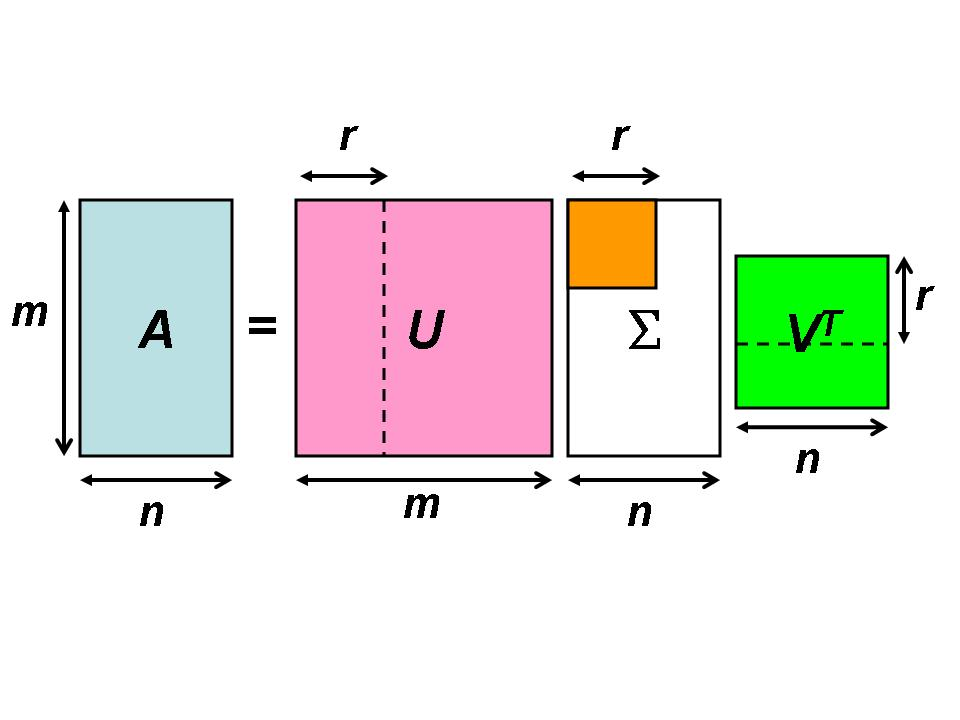
\includegraphics[scale=0.2]{SVD.jpg}
	\caption{tSVD分解}
	\label{1}
\end{figure}
\section{线性变换}
\subsection{线性相关}
\subsection{特征值与特征向量}
\subsection{线性代数几何意义}
正交矩阵


\section{误差分析}





\section{特殊函数}



\section{偏微分方程}


\section{玻尔兹曼分布}
\chapter{数理统计基础}
\section{概率}

1. 概率的定义(略)概率满足:非负性,规范性,可列可加性

2. 概率的性质:

   ​	重点:逆事件概率;加法公式;有限可加性

3. 条件概率:
\begin{equation}
    P(A|B)=\frac{P(AB)}{P(B)}
\end{equation}

4. 乘法定理:
\begin{equation}
    P(AB)=P(A|B)P(A)
\end{equation}

5. 全概率公式:
\begin{equation}
    P(A)=P\left(A \mid B_{1}\right) P\left(B_{1}\right)+
    P\left(A \mid B_{2}\right) P\left(B_{2}\right)+\ldots+
    P\left(A \mid B_{n}\right) P\left(B_{n}\right)
\end{equation}

6. 独立性:满足
\begin{subequations}
    \begin{align}
        P(AB)&=P(A)P(B) \\ 
        P(B|A)&=P(B)\\
    \end{align}
\end{subequations}

 \section{单变量分布}
 1. 随机变量的概念(略)

 2. 分布函数的概念(略)和性质:不减函数;$0\leq F(x)\leq 1 $; $F(x+0)=F(x)$
 
 3. 概率密度函数
 \begin{equation}
    F(x)=\int_{-\infty}^{x}f(t) \rm dt
\end{equation}
 
 性质:
\begin{subequations}
\begin{align}
    f(x)&\leq 0 \\ 
    \int_{-\infty}^{\infty}f(x)dx&=1\\
    P\{x_1<X<x_2\}&=\int_{x_1}^{x_2}f(x)dx\\
    F'(x)&=f(x)
\end{align}
\end{subequations}

\section{常见分布}
1. (0-1)分布:
\begin{equation}
    P(X=k)=p^{k}(1-p)^{1-k}, 0<p<1, k=0,1
\end{equation}

2. 二项分布: 
\begin{equation}
    P(X=k)=\left(\begin{array}{l}n \\k\end{array}\right) p^{k}(1-p)^{n-k}
\end{equation}

3. 泊松分布: 
\begin{equation}
    P(X=k)=\frac{\lambda^{k} e^{-\lambda}}{k !}, k=0,1,2, \ldots
\end{equation}

4. Beta分布: 
   \begin{equation}
    f(x)=\frac{\Gamma(\alpha+\beta)}{\Gamma(\alpha) \Gamma(\beta)} x^{\alpha-1}(1-x)^{\beta-1}
   \end{equation}
   
   其中:$0\leq x\leq 1, \ \alpha>0,\ \beta>0,\ \Gamma(z)=\int_{0}^{+\infty} t^{z-1} e^{-t} d t$

5. 均匀分布: 
   \begin{equation}
        f(x)=\left\{\begin{array}{ll}\frac{1}{b-a} & a<x<b \\0 & \text { otherwise }\end{array}\right.
   \end{equation}
   
6. 指数分布: 
\begin{equation}
    f(x)=\left\{\begin{array}{ll}\frac{1}{\theta} e^{-x / \theta} & x>0 \\0 & \text { otherwise }\end{array}\right.
\end{equation}

7. 正态分布: 
\begin{equation}
    f(x)=\frac{1}{\sqrt{2 \pi} \sigma} e^{-\frac{(x-\mu)^{2}}{2 \sigma^{2}}}
\end{equation}
   $f(x)$关于$\mu$对称;$f(\mu)=max(f(x))=\frac{1}{\sqrt{2\pi}\sigma}$。

8. $Gamma$分布: 
\begin{equation}
   f(x)=\frac{\beta^{\alpha}}{\Gamma(\alpha)} x^{\alpha-1} e^{-\beta x}
\end{equation}
   其中:$x>0,\ \alpha>0,\ \beta>0$

9. Inv-$Gamma$分布: 
\begin{equation}
    f(x)=\frac{\beta^{\alpha}}{\Gamma(\alpha)} x^{-(\alpha+1)} e^{-\frac{\beta}{x}}
\end{equation}
   其中:$x>0,\ \alpha>0,\ \beta>0$

10. $\chi ^2$分布: 
\begin{equation}
    f_{k}(x)=\frac{1}{2^{\frac{k}{2}} \Gamma\left(\frac{k}{2}\right)} x^{\frac{k}{2}-1} e^{-\frac{x}{2}}
\end{equation}
    等价$\alpha=k/2,\beta = 1/2$的Gamma分布

11. Inv-$\chi ^2$分布: 
\begin{equation}
    f(x)=\frac{2^{-\frac{k}{2}}}{\Gamma\left(\frac{k}{2}\right)} x^{-\left(\frac{k}{2}+1\right)} e^{-\frac{1}{2 x}}
\end{equation}
    
    等价$\alpha=k/2,\beta = 1/2$的Inv-Gamma分布

12. Scaled Inv-$\chi ^2$分布: 
   \begin{equation}
       f(x)=\frac{\frac{k}{2}^{-\frac{k}{2}} s^{k}}{\Gamma\left(\frac{k}{2}\right)} x^{-\left(\frac{k}{2}+1\right)} e^{-\frac{k s^{2}}{2 x}}
   \end{equation}
     等价$\alpha=k/2,\beta = ks^2/2$的Inv-Gamma分布。


\section{多元随机变量}

\section{随机变量的数学特征}

\section{频率学派的参数估计}

\section{频率学派的假设检验}
\chapter{贝叶斯统计}
\section{贝叶斯定理}
1. 贝叶斯公式
\begin{equation}
    P(B_i|A)=\frac{P(A|B_i)P(B_i)}{\sum_{j=1}^{n}P(A|B_i)P(B_j)}
    =\frac{P(A|B_i)P(B_i)}{P(A)}
\end{equation}
先验:$P(B)$

似然:  $P(A|B)$

后验:  $P(B|A)$

证据(归一化):  $P(A)$

2. 贝叶斯公式含义:通过数据推算模型参数的概率。即:
\begin{equation}
    P({\rm{Model}} (\theta)|{\rm{Data}})=
    P({\rm{Data}}|{\rm{Model}}(\theta))P(\theta)
\end{equation}


3. 贝叶斯统计的优势:将这个某种程度上是主观性的信息明确表达在先验概率中,而不是隐藏在没有明确指出的假设中; 让数据说话,减少主观性的先验概率。
%单变量贝叶斯参数估计
\section{贝叶斯单参数估计}
\subsection{二项分布估计}

\subsubsection{\textbf{无信息先验}}

\begin{itemize}
\item
  似然:
\end{itemize}

\begin{equation} 
p(y|\theta)=
\left(                 
  \begin{array}{ccc}   
    n\\ 
    y\\  
  \end{array}
\right)                 
\theta^y(1-\theta)^{n-y}
\end{equation}

\begin{itemize}
\item
  先验:均匀分布
\item
  后验:
\end{itemize}

\begin{equation}
  p(\theta|y)\propto\theta^y(1-\theta)^{n-y}\sim Beta(y+1,n-y+1)
\end{equation}

\begin{itemize}
\item
  预测:
\end{itemize}

\begin{equation}
  Pr(\widetilde y=1|y)=\int_0^1Pr(\widetilde y=1|\theta,y)
  =\int_0^1\theta p(\theta|y)d\theta=E(\theta|y)
\end{equation}

\subsubsection{\textbf{有信息先验}}

\begin{itemize}
\item
  先验:\(p(\theta)\propto \theta^{\alpha-1}(1-\theta)^{\beta-1}\)
\item
  似然:
\end{itemize}
\begin{equation}      
p(y|\theta)=
\left(                 
  \begin{array}{ccc}   
    n\\ 
    y\\  
  \end{array}
\right)                 
\theta^y(1-\theta)^{n-y}
\end{equation}

\begin{itemize}
\item
  后验:
\end{itemize}

\[p(\theta|y)\propto \theta^{y+\alpha-1}(1-\theta)^{n-y+\beta-1}\sim Beta(\alpha+y,\beta+n-y)\]

\begin{itemize}
\item
  后验期望:\(E(\theta|y)=\frac{\alpha+y}{\alpha+\beta+n}\)
\item
  先验期望:\(E(y)=\frac{\alpha}{\alpha+\beta}\)
\end{itemize}

当\(n\rightarrow\infty\): \(E(\theta|y)\rightarrow y/n\)

数据很大的时候可以用正态分布近似后验分布

\subsection{正态分布参数估计}

\begin{enumerate}
\def\labelenumi{\arabic{enumi}.}
\item
  \textbf{已知方差求均值}
\end{enumerate}

\begin{itemize}
\item
  似然:
\end{itemize}

\begin{equation}
  p(y|\theta)=\frac{1}{\sqrt{2\pi\sigma^2}}
  \exp\left[-\frac{1}{2\sigma^2}(y-\theta)^2\right]
  \sim N(\theta,\sigma^2)
\end{equation}


\begin{itemize}
\item
  先验:

\begin{equation}
  p(\theta)\propto\exp\left(-\frac{1}{2\tau_0^2}(\theta-\mu_0)^2\right)
  \sim N(\mu_0,\tau_0^2)
\end{equation}
\item
  后验:

\begin{equation}
  p(\theta|y)
  \propto\exp\left(-\frac{1}{2\tau_1^2}(\theta-\mu_1)^2\right)
  \sim N(\mu_1,\tau_1)
\end{equation}

  其中:

  \[\mu_1=\frac
  {\frac{1}{\tau_0^2}\mu_0+\frac{1}{\sigma^2}y}
  {\frac{1}{\tau_0^2}+\frac{1}{\sigma^2}}\]

  \[\frac{1}{\tau_1^2}=\frac{1}{\tau_0^2}+\frac{1}{\sigma^2}\]

  精度:方差的倒数
\item
  预测:

\begin{equation}
  \begin{aligned}
    p(\widetilde y|y)&=\int p(\widetilde y | \theta)p(\theta|y)d\theta\\
    &\propto
    \int\exp\left(-\frac{(\widetilde y - \theta)^2}{2\sigma^2}\right)
    \exp \left(-\frac{(\theta-\mu_1)^2}{2\tau_1^2}\right)d\theta\\
    E(\widetilde y|\theta)&=\theta\\
    D(\widetilde y|\theta)&=\sigma^2+\tau^2_1
    \end{aligned}
\end{equation}

\item
  多个相互独立数据:
\end{itemize}


\begin{equation}
  \begin{aligned}
  p(\theta \mid y) & \propto p(\theta) p(y \mid \theta) 
  \\&=p(\theta) \prod_{i=1}^{n} p\left(y_{i} \mid \theta\right) 
  \\& \propto \exp \left(-\frac{1}{2 \tau_{0}^{2}}\left(\theta-\mu_{0}\right)^{2}\right) \prod_{i=1}^{n} \exp \left(-\frac{1}{2 \sigma^{2}}\left(y_{i}-\theta\right)^{2}\right) 
  \\& \propto \exp \left(-\frac{1}{2}\left[\frac{1}{\tau_{0}^{2}}\left(\theta-\mu_{0}\right)^{2}+\frac{1}{\sigma^{2}} \sum_{i=1}^{n}\left(y_{i}-\theta\right)^{2}\right]\right)
  \end{aligned}
\end{equation}
可得:

\[p(\theta|y_1,\cdots,y_n)=p(\theta|\bar y)=N(\theta | \mu_n,\tau_n^2)\]

其中:

\[\mu_{n}=\frac{\frac{1}{\tau_{0}^{2}} \mu_{0}+\frac{n}{\sigma^{2}} \bar{y}}{\frac{1}{\tau_{0}^{2}}+\frac{n}{\sigma^{2}}}\]

\[\frac{1}{\tau_{n}^{2}}=\frac{1}{\tau_{0}^{2}}+\frac{n}{\sigma^{2}}\]

若\(n\rightarrow+\infty\),\(\tau_0\)不变,则:\(\theta|y\sim N(\bar{y},\sigma^2/n)\)

若\(\tau\rightarrow+\infty\),\(n\)
不变,则:\(\theta|y\sim N(\bar{y},\sigma^2/n)\)

\begin{enumerate}
\def\labelenumi{\arabic{enumi}.}
\item
  \textbf{已知均值求方差}
\end{enumerate}

由于有\(n\)个服从\(\sim N(\theta,\sigma^2)\)的分布,因此:

\begin{itemize}
\item
  似然:
\end{itemize}

\begin{equation}
  p(y|\sigma^2)\propto\sigma^{-n}\exp\left(-
\frac{1}{2\sigma^2}\sum_{i=1}^{n}(y_i-\theta)^2
\right)=(\sigma^2)^{-n/2}e^{-\frac{n}{2\sigma^2}v}
\end{equation}


其中:

\[v=\frac{1}{n}\sum_{i=1}^n(y_i-\theta)^2\]

\begin{itemize}
\item
  共轭先验:\(p(\sigma^2)\propto(\sigma^2)^{-\alpha+1}e^{\beta/\sigma^2} \sim \rm Inv-\chi^2(\upsilon_0,\sigma^2_0)\)
\item
  后验:
\end{itemize}

\begin{equation}
    \begin{aligned}
        p(\sigma^2|y)&\propto p(\sigma^2)p(y|\sigma^2)\\
        &\propto \left( \frac{\sigma^2_0}{\sigma^2} \right)^{v_0/2+1}
        \exp\left( -\frac{\upsilon_0\sigma^2_0}{2\sigma^2} \right)\cdot
        (\sigma^2)^{-n/2}\exp\left(-\frac{n}{2}\frac{\upsilon}{\sigma^2}\right)\\
        &\propto (\sigma^2)^{-((n+\upsilon_0)/2+1)}\exp\left(
        -\frac{1}{2\sigma^2}(\upsilon_0\sigma_0^2+n\upsilon)
        \right)\\
        &\sim \textrm{Inv}-\chi^2(\upsilon_0+n,\frac{\upsilon_0\sigma_0^2+n\upsilon}{\upsilon_0+n})
        \end{aligned}
\end{equation}

%多变量贝叶斯参数估计
\section{贝叶斯多参数模型}
\subsubsection{一、多参数模型处理}

\begin{enumerate}
\def\labelenumi{\arabic{enumi}.}
\item
  \textbf{置之不理}
\item
  \textbf{边缘化}
\begin{equation}
  p(\theta_1|y)=\int p(\theta_1,\theta_2|y)d\theta_2
\end{equation}
  
  用贝叶斯公式展开:

  \[p(\theta_1,\theta_2|y)\propto p(y|\theta_1,\theta_2)p(\theta_1,\theta_2)\]

  将\(\theta_2\)边缘化积分,得到\(\theta_1\)的后验分布。
\item
  \textbf{平均化}

  \[p(\theta_1|y)=\int p(\theta_1|\theta_2,y)p(\theta_2|y)d\theta_2\]
\end{enumerate}

\hypertarget{ux4e8cux65e0ux4fe1ux606fux5148ux9a8cux7684ux6b63ux6001ux5206ux5e03}{%
\subsubsection{二、无信息先验的正态分布}\label{ux4e8cux65e0ux4fe1ux606fux5148ux9a8cux7684ux6b63ux6001ux5206ux5e03}}

\begin{itemize}
\item
  先验:

  \[p(\mu,\ln\sigma^2)\sim U(\mu,\ln \sigma^2)\]

  或者先验写为:

  \[p(\mu,\sigma^2)\sim\frac{1}{\sigma^2}\]
\item
  似然 ( \textbf{有\(n\)次观测 }) :

  \[p(y|\mu,\sigma^2)=\sigma^{-n}\exp \left(
  -\frac{1}{2\sigma^2}\sum_{i=1}^{n}(y_i-\mu)^2
  \right)\]
\item
  联合后验:

  \[p(\mu,\sigma^2|y)\propto \sigma^{-n-2}\exp\left(
  -\frac{1}{2\sigma^2}[(n-1)s^2+n(\bar{y}-\mu)^2]
  \right)\]

  其中:

  \[s^2=\frac{1}{n-1}\sum_{i=1}^{n}(y_i-\bar y)^2\]
\item
  边缘后验\(p(\sigma^2|y)\):

  \begin{align*}
  p(\sigma^2|y)
  &\propto \int p(\mu,\sigma^2|y)d\mu\\
  &\propto(\sigma^2)^{-\frac{n+1}{2}}\exp\left(
  -\frac{(n-1)s^2}{2\sigma^2}
  \right)\\
  &\sim Inv-\chi^2(n-1,s^2)
  \end{align*}
\item
  边缘后验\(p(\mu|y)\):

  \begin{align*}
  p(\mu|y)
  &=\int_0^{\infty}p(\mu,\sigma^2|y)d\sigma^2\\
  &\propto\left[
  1+\frac{n(\mu-\bar y)^2}{(n-1)s^2}^{-n/2}
  \right] \\
  &\sim t_{n-1}(\bar y,s^2/n)
  \end{align*}
\item
  预测后验分布

  \[p(\widetilde y|y)=\iint  p(\widetilde y |\mu,\sigma^2,y)p(\mu,\sigma^2|y)
  d\mu d\sigma^2\]
\end{itemize}

\hypertarget{ux4e09ux5171ux8f6dux5148ux9a8cux5206ux5e03}{%
\subsubsection{三、共轭先验分布}\label{ux4e09ux5171ux8f6dux5148ux9a8cux5206ux5e03}}

\begin{itemize}
\item
  先验分布:

  \(\mu|\sigma^2 \sim N(\mu_0,\sigma^2/\kappa_0)\)

  \(\sigma^2 \sim Inv-\chi^2(\nu_0,\sigma^2_0)\)
\item
  联合先验分布

  \begin{align*}
  p(\mu,\sigma^2)
  &=p(\mu|\sigma^2)p(\sigma^2)\\
  &\propto N-Inv-\chi^2(\mu_0,\sigma^2_0/\kappa_0\ ;\ \nu_0,\sigma^2_0 )
  \end{align*}
\item
  似然分布

  \[p(y|\mu,\sigma^2)=\sigma^{-n}\exp \left(
  -\frac{1}{2\sigma^2}\sum_{i=1}^{n}(y_i-\mu)^2
  \right)\]
\item
  联合后验分布
\begin{equation}
  \begin{aligned}
    p\left(\mu, \sigma^{2} \mid y\right) 
    & \propto \sigma^{-1}\left(\sigma^{2}\right)^{\left(\nu_{0} / 2+1\right)} e^{-\frac{1}{2 \sigma^{2}}\left[\nu_{0} \sigma_{0}^{2}+\kappa_{0}\left(\mu-\mu_{0}\right)^{2}\right]}
    \left(\sigma^{2}\right)^{-n / 2} e^{-\frac{1}{2 \sigma^{2}}\left[(n-1) s^{2}+n(\bar{y}-\mu)^{2}\right]} \\
    & \propto \mathrm{N}-\operatorname{Inv}-\chi^{2}\left(\mu_{n}, \sigma_{n}^{2} / \kappa_{n} ; \nu_{n}, \sigma_{n}^{2}\right)
  \end{aligned}
\end{equation}


\end{itemize}

其中参数为:
\begin{equation}
  \begin{array}{c}
    \mu_{n}   = \frac{\kappa_{0}}{\kappa_{0}+n} \mu_{0}+\frac{n}{\kappa_{0}+n} \bar{y}\\
    \kappa_{n}= \kappa_{0}+n \\
    \nu_{n}   = \nu_{0}+n \\
    \nu_{n} \sigma_{n}^{2}=\nu_{0} \sigma_{0}^{2}+(n-1) s^{2}+\frac{\kappa_{0} n}{\kappa_{0}+n}\left(\bar{y}-\mu_{0}\right)^{2}
    \end{array}
\end{equation}


\begin{itemize}
\item
  条件后验分布\(p(\mu|\sigma^2,y)\)
\end{itemize}

\[(\mu \mid \sigma^{2}, y) \sim \mathrm{N}\left(\mu_{n} \frac{\sigma^{2}}{\kappa_{n}}\right)\]

\begin{itemize}
\item
  方差边缘后验分布\(p(\sigma^2|y)\)
\end{itemize}

\[(\sigma^{2} \mid y) \sim \operatorname{Inv}-\chi^{2}\left(\nu_{n}, \sigma_{n}^{2}\right)\]

\begin{itemize}
\item
  均值边缘后验分布\(p(\mu|y)\)
\end{itemize}

\begin{equation}
  \begin{aligned}
    p(\mu \mid y) 
    & \propto\left[1+\frac{\kappa_{n}\left(\mu-\mu_{n}\right)^{2}}{\nu_{n} \sigma_{n}^{2}}\right]^{-\left(\nu_{n}+1\right) / 2} \\
    & = t_{\nu_{n}}\left(\mu \mid m u_{n}, \sigma_{n}^{2} / \kappa_{n}\right)
  \end{aligned}
\end{equation}

%分层贝叶斯模型
\section{Chapter 5层次化模型}

\subsubsection{一、参数化先验分布}
\begin{enumerate}
\def\labelenumi{\arabic{enumi}.}
\item
  先验分布

  先验分布是由某个未知参数的分布\(\phi\)给出:

  \[p(\theta|\phi)=\prod_{j=1}^Jp(\theta_j|\phi)\ \ \ \ \  \theta=(\theta_1,\theta_2,\cdots)\]

  边缘化:

  \[p(\theta)=\int\left( \prod_{j=1}^Jp(\theta_j|\phi) \right)p(\phi)d\phi\]
\item
  联合先验分布 \(p(\phi,\theta)=p(\theta|\phi)p(\phi)\)
\item
  超先验分布 : \(p(\phi)\)
\item
  后验分布

  \begin{itemize}
  \item
    联合后验 : \(p(\phi,\theta|y)=p(y|\theta)p(\theta|\phi)p(\phi)\)
  \item
    条件后验:\(p(\theta|\phi,y)\)
  \item
    边缘后验:\(p(\phi|y)\)

    \[p(\phi|y)=\frac{p(\theta,\phi|y)}{p(\theta|\phi,y)}\]
  \end{itemize}
\item
  层次化贝叶斯完整表述
\end{enumerate}

\begin{equation}
  \begin{aligned}
    p(\phi,\theta|y)
    &\propto p(y|\phi,\theta)p(\phi,\theta)\\
    &=p(y|\theta)p(\phi,\theta)\\
    &=p(y|\theta)p(\theta|\phi)p(\phi)
    \end{aligned}
\end{equation}


\begin{enumerate}
\def\labelenumi{\arabic{enumi}.}
\item
  层次化贝叶斯计算步骤
\end{enumerate}

\begin{itemize}
\item
  写出联合后验分布\(p(\theta,\phi|y)\):即超先验分布,总体分布和似然分布的乘积
\item
  确定条件后验分布\(p(\theta|\phi,y)\):

  \[p(\theta|\phi,y)=\prod_{j=1}^J p(\theta_j|\phi,y)\]
\item
  边缘化给出\(\phi\)的贝叶斯估计
\end{itemize}

\hypertarget{ux4e8cux4e8cux9879ux5206ux5e03ux7684ux5206ux5c42ux8d1dux53f6ux65afux6a21ux578b}{%
\subsubsection{二、二项分布的分层贝叶斯模型}\label{ux4e8cux4e8cux9879ux5206ux5e03ux7684ux5206ux5c42ux8d1dux53f6ux65afux6a21ux578b}}

\begin{enumerate}
\def\labelenumi{\arabic{enumi}.}
\item
  \(y_i\)先验(组内模型) \(y_j \sim Bin(n_j,\theta_j)\)
\item
  \(\theta_j\)先验(组间模型):\(\theta_j\sim Beta(\alpha,\beta)\)
\item
  联合先验:\(p(\alpha,\beta,\theta)=p(\alpha,\beta)p(\theta|\alpha,\beta)\)
\item
  似然:\(p(y|\theta,\alpha,\beta)\)
\item
  联合后验:\(p(\theta,\alpha,\beta|y)\)

\begin{equation}
  \begin{aligned}
    p(\theta,\alpha,\beta|y)
    &\propto p(\alpha,\beta)p(\theta|\alpha,\beta)p(y|\theta,\alpha,\beta)\\
    &=p(\alpha,\beta)\prod_{j=1}^{J}
    \frac{\Gamma(\alpha+\beta)}{\Gamma(\alpha)\Gamma(\beta)}
    \theta_j^{\alpha-1}(1-\theta_j)^{\beta-1}
    \prod_{j=1}^{J}
    \theta_j^{y_j}(1-\theta_j)^{n_j-y_j}
    \end{aligned}
\end{equation}

\item
  条件后验: \(p(\theta|\alpha,\beta,y)\) : 单参数模型给定的后验

\begin{equation}
  \begin{aligned}
    p(\theta \mid \alpha, \beta, y)
    &=\prod_{j=1}^{J} \frac{\Gamma\left(\alpha+\beta+n_{j}\right)}{\Gamma\left(\alpha+y_{j}\right) \Gamma\left(\beta+n_{j}-y_{j}\right)} 
    \theta_{j}^{\alpha+y_{j}-1}\left(1-\theta_{j}\right)^{\beta+n_{j}-y_{j}-1}\\
    &\sim \prod _{j=1}^JBeta(\alpha+y_j,\beta+n_j-y_j)
    \end{aligned}
\end{equation}

\item
  边缘后验:\(p(\alpha,\beta|y)\)
\begin{equation}
  \begin{aligned}
    p(\alpha, \beta \mid y)
    =& \frac{p(\theta, \alpha, \beta \mid y)}{p(\theta \mid \alpha, \beta, y)} \\
    &\propto \frac{p(\alpha, \beta) \prod_{j=1}^{J} 
    \frac{\Gamma(\alpha+\beta)}{\Gamma(\alpha) \Gamma(\beta)} 
    \theta_{j}^{\alpha-1}\left(1-\theta_{j}\right)^{\beta-1} \prod_{j=1}^{J} \theta_{j}^{y_{j}}\left(1-\theta_{j}\right)^{n_{j}-y_{j}}}{\prod_{j=1}^{J} 
    \frac{\Gamma\left(\alpha+\beta+n_{j}\right)}{\Gamma\left(\alpha+y_{j}\right) \Gamma\left(\beta+n_{j}-y_{j}\right)} 
    \theta_{j}^{\alpha+y_{j}-1}\left(1-\theta_{j}\right)^{\beta+n_{j}-y_{j}-1}} \\
    =& p(\alpha, \beta) \prod_{j=1}^{J} \frac{\Gamma(\alpha+\beta) \Gamma\left(\alpha+y_{j}\right) 
    \Gamma\left(\beta+n_{j}-y_{j}\right)}{\Gamma(\alpha) \Gamma(\beta) \Gamma\left(\alpha+\beta+n_{j}\right)}
    \end{aligned}
\end{equation}

\end{enumerate}

\hypertarget{ux4e09ux6b63ux6001ux5206ux5e03ux7684ux5206ux5c42ux8d1dux53f6ux65afux6a21ux578b}{%
\subsubsection{三、正态分布的分层贝叶斯模型}\label{ux4e09ux6b63ux6001ux5206ux5e03ux7684ux5206ux5c42ux8d1dux53f6ux65afux6a21ux578b}}

\begin{enumerate}
\def\labelenumi{\arabic{enumi}.}
\item
  \textbf{数据结构}
\end{enumerate}

假设\(J\)个独立试验,每个实验都由\(\theta_j\)给出其参数估计,估计\(n_j\)个\(i.i.d\)正态分布的数据点\(y_{ij}\),每个点方差为\(\sigma^2\):

\[y_{i j} | \theta_{j} \sim N\left(\theta_{j}, \sigma^{2}\right) \quad i=1, \ldots, n_{j} \quad j=1, \ldots, J\]

样本均值(充分统计量):

\[\bar{y}_{\cdot j}=\frac{1}{n_j}\sum_{i=1}^{n_j}y_{ij}\]

样本均值的分布

\[\bar y_{\cdot j} \sim N(\theta_j,\sigma^2_j)\]

样本方差:

\[\sigma^2_j=\frac{\sigma^2}{n_j}\]

样本的均值是从\(\theta\)中估计,样本方差是从\(\sigma\)中估计。

相当于 \(\theta\) 的似然分布:

\[\bar y_{\cdot j}|\theta \sim N(\theta_j,\sigma^2_j)\]

由于 \(\sigma\) 是已知的,下面所有的分布都是在 \(\sigma\)
已知情况下成立。

\begin{enumerate}
\def\labelenumi{\arabic{enumi}.}
\item
  \textbf{层次化模型:无信息先验}
\end{enumerate}

\(\theta\)是从参数\((\mu,\tau)\)中抽取:

\[p\left(\theta_{1}, \ldots, \theta_{J} \mid \mu, \tau^{2}\right)=\prod_{j=1}^{J} p\left(\theta_{j} \mid \mu, \tau^{2}\right)\]

边缘化:

\[p\left(\theta_{1}, \ldots, \theta_{J}\right)=
\iint \prod_{j=1}^{J}
\left[p\left(\theta_{j} \mid \mu, \tau^{2}\right)\right] 
p\left(\mu, \tau^{2}\right)
d \mu d \tau\]

\begin{itemize}
\item
  \textbf{先验和似然}
\end{itemize}

组内抽样:\(\bar y_{\cdot j} \sim N(\theta_j,\sigma^2_j)\)

\(\theta\)的先验(组内模型):\(\theta|\mu,\tau \sim N(\mu,\tau^2)\)

\(\mu\)的先验: \(p(\mu,\tau)=p(\mu|\tau)p(\tau)\propto p(\tau)\)

\(\theta_j\)似然分布:\(p(y|\theta)\sim(\bar y_{\cdot j}|\theta) \sim N(\theta_j,\sigma^2_j)\)

\begin{itemize}
\item
  \textbf{联合后验:}\(p(\theta,\phi|y)\)
\end{itemize}

\begin{equation}
  \begin{aligned}
    p(\theta,\mu,\tau|y)
    &\propto p(\mu,\tau)p(\theta|\mu,\tau)p(y|\theta)\\
    &\propto p(\mu,\tau)\prod_{j=1}^{J}p(\theta_j|\mu,\tau^2)
    \prod_{j=1}^{J}p(\bar y _{\cdot j}|\theta_j,\sigma^2_j)
    \end{aligned}
\end{equation}


其中:\(\bar y _{\cdot j}\sim N(\theta_j,\sigma_j^2)\)

可以忽略只依赖 \(y\) 和 \(\sigma_j\) 的参数,因为其已知。

\begin{itemize}
\item
  \textbf{\(\theta\)条件后验:}\(p(\theta_{j} \mid \mu, \tau, y_{\cdot, j})\)
\end{itemize}

\[\theta_{j} \mid \mu, \tau, y_{\cdot, j} \sim N\left(\hat{\theta}_{j}, V_{j}\right)\]

其中:

\[\hat{\theta}_{j}=
\frac
{\frac{1}{\sigma_{j}^{2}} \bar{y}_{\cdot j}+
\frac{1}{\tau^{2}} \mu}
{\frac{1}{\sigma_{j}^{2}}+\frac{1}{\tau^{2}}}\]

\[V_{j}=\frac{1}{\frac{1}{\sigma_{j}^{2}}+\frac{1}{\tau^{2}}}\]

\begin{itemize}
\item
  \textbf{超参数边缘后验:}\(p(\mu, \tau \mid y)\)
\end{itemize}

\[p(\mu, \tau \mid y) \propto p(\mu, \tau) p(y \mid \mu, \tau)\]

对于正态分布:

\[\bar{y}_{\cdot j}\sim N(\mu,\tau^2+\sigma^2)\]

因此:

\[p(\mu, \tau \mid y) \propto p(\mu, \tau) \prod_{j=1}^{J} p\left(\bar{y} _{\cdot j} \mid \mu, \tau^{2}+\sigma_{j}^{2}\right)\]

\[\bar{y}_{\cdot j} \mid \mu, (\tau^{2}+\sigma_{j}^{2}) 
\sim
N \left( \mu, \tau^{2} + \sigma_{j}^{2} \right)\]

\begin{itemize}
\item
  \textbf{给定\(\tau\)下\(\mu\)的边缘后验分布}:
  \(p(\mu \mid \tau, y)\)从单参数模型中得出的结论
\end{itemize}

\begin{equation}
  \begin{array}{c}
    \mu \mid \tau, y \sim N\left(\hat{\mu}, V_{\mu}\right) \\
    \end{array}
\end{equation}


\[\hat{\mu}=\frac{\sum_{j=1}^{J} \frac{1}{\sigma_{j}^{2}+\tau^{2}} \bar{y}_{\cdot j}}{\sum_{j=1}^{J} \frac{1}{\sigma_{j}^{2}+\tau^{2}}}\]

\[\\V_{\mu}^{-1}=\sum_{j=1}^{J} \frac{1}{\sigma_{j}^{2}+\tau^{2}}\]

\begin{itemize}
\item
  \(\tau\)的后验:\(p(\tau \mid y) \)
\end{itemize}

\begin{equation}
  \begin{aligned}
    p(\tau \mid y) 
    &=\frac{p(\mu, \tau \mid y)}{p(\mu \mid \tau, y)} \\
    &\propto 
    \frac{p(\tau) \prod_{j=1}^{J} 
    N\left(\bar{y}_{ \cdot j }\mid \mu, \sigma_{j}^{2}+\tau^{2}\right)}
    {N\left(\mu \mid \hat{\mu}, V_{\mu}\right)} \\
    & \propto p(\tau) V_{\mu}^{1 / 2} 
    \prod_{j=1}^{J}\left(\sigma_{j}^{2}+\tau^{2}\right)^{-1 / 2} 
    \exp \left(
    -\frac{\left(\bar{y}_{\cdot j}-\hat{\mu}\right)^{2}}{2\left(\sigma_{j}^{2}+\tau^{2}\right)}
    \right)
    \end{aligned}
\end{equation}


\begin{itemize}
\item
  从后往前采样,即先算出\(\tau\)的后验,然后依次采样算出\(\mu\)的后验,超参数联合后验,\(\theta\)的条件后验,联合后验等。
\end{itemize}

\section{贝叶斯回归}

\section{贝叶斯模型选择}
\section{费舍尔信息矩阵Fisher Information}
\chapter{傅里叶变换}
\section{傅里叶级数与傅里叶变换}

\section{拉普拉斯变换}

\section{均匀采样与离散傅里叶变换}

\section{非均匀采样下的周期检测}

\section{快速傅里叶变换及其matlab和python实现}


\chapter{随机过程}
\section{随机过程及其统计描述}

\section{平稳随机过程}

\section{马尔科夫链}


\chapter{MCMC与采样方法}
\section{蒙特卡罗法 Monte Carlo Method}

\subsection{随机采样和接受-拒绝采样}

蒙特卡罗法是通过概率模型的随机抽样进行随机抽样的方法。假设概率分布已知,通过概率分布得到随机样本,并通过得到的随机样本得到概率分布的随机性质,因此蒙特卡洛方法的核心是随机抽样。接下来我们介绍\textbf{接受-拒绝采样}。

已知概率密度分布为\(f(x)\),但是这个概率密度分布复杂,各个变量并不独立,无法直接采样或者积分,因此可以通过蒙特卡罗方法进行抽样,得到样本\emph{\(X\)},得到其随机分布。我们在这介绍\textbf{接受-拒绝采样}。我们需要一个辅助的\textbf{建议分布},记为\(q(x)\)。这个建议分布可以产生我们的候选样本,但建议分布要满足:

\[c * q(x) \geq f(x)\]

之后我们对样本按照建议分布\(q(x)\)进行抽样,得到样本\(x^*\),同时对均匀分布\(U(0,1)\)进行抽样,得到\(u\)。之后计算\(\frac{f(x)}{c*q(x)}\)(这个值一定在0\textasciitilde1之间,对应图1的绿色部分比例),若

\[u \leq \frac{f(x^*)}{c*q(x^*)}\]

则\(x^*\)接受作为样本,否则拒绝。

怎么理解这个过程呢?简单来说就是我们先对建议分布\(q(x)\)的概率密度进行采样,因为这个比我们的\(f(x)\)更容易采样。假如这个分布很复杂,维度很高,直接算的话浪费计算资源,因此要先用一个简单的建议分布\(q(x)\)进行采样,得到建议的采样,但是这建议分布的采样终究不是我们需要的采样,所以我们需要在利用均匀分布\(U(0,1)\),由我们算出来的\(f(x^*)/cq(x^*)\)进行接受或者拒绝。在图1中,按照绿色比例进行接受。如果在第\(x^*_i\)个抽样刚好落在中间红色区域比较大的点,那么拒绝的概率就高,反之绿色部分的比例更大,则我们接受的概率就越高。

\begin{figure}
\centering
%\includegraphics{C:/Users/astro_gh/Desktop/QQ图片20201119220859.jpg}
\caption{}
\end{figure}

听到这是不是有点迷糊了?别着急!我们看看图1,在是不是\(x^*\)处红色部分占比越大,与目标分布\(f(x)\)相差就越远了?所以我们在这里就必须剔除一些点了,不然远离我们的真实分布了!
这时候可能会有其他疑问了,那在图1两端概率很小时候岂不是都接受率很高?是的,但是那两端概率很低呀!因为我们在使用建议分布抽样的时候概率那里的点已经是很少了,所以我们不用拒绝很多样本点也就和目标分布类似了。
所以这时候就要用到一个均匀分布\(U(0,1)\),在该点上随机生成一个\(u\),然后按照\((1.1)\)则接受,否则拒绝。

所以假设我们抽了n个样本,对样本进行拒绝,就是要生成和判断n次\(u\)的取值,也就是对每个样本点进行计算和判断是否拒绝,完成一次拒绝-接受采样。

接受-拒绝采样的缺点也是有的,主要是接受率比较低,抽样效率低。
\subsection{数学期望和蒙特卡罗积分}
如果我们要算目标函数为\(f(x)\),其概率密度为\(p(x)\),我们记函数\(f(x)\)关于密度函数\(p(x)\)的数学期望为\(E_{p(x)}[f(x)]\)。我们按照密度函数\(f(x)\)独立抽取n个样本\(x_1,x_2\cdots,x_n\),之后计算样本的均值:

\[\hat{f}_n=\frac{1}{n}\sum_{i=1}^{n}f(x_i)\]

作为\(f(x)\)的近似值。根据大数定理,当样本容量增大,样本均值以概率1收敛于数学期望。因此我们可以用上述方法得到我们的数学期望。

\[E_{p(x)}[f(x)]\approx\frac{1}{n}\sum_{i=1}^{n}f(x_i)\]

而在\(\mathcal{X}\)上数学期望的积分形式为:

\[E(x)=\int_{\mathcal{X}} f(x)p(x)dx\]

如果我们的目标积分为:

\[h(x)=f(x)q(x)\]

我们可以写为:

\[\int_{\mathcal{X}}h(x)dx=\int_{\mathcal{X}}f(x)q(x)dx=E_{p(x)}[f(x)]\]

对于复杂的函数,可以给定一个概率密度函数\(p(x)\),只要取

\[f(x)=\frac{h(x)}{p(x)}\]

就可以用\(p(x)\)进行抽样算出积分:

\[\int_{\mathcal{X}}h(x)dx=E_{p(x)}[f(x)]\approx\frac{1}{n}\sum_{i=1}^{n}f(x_i)\]

因此我们可以先用\(p(x)\)抽样。然后再进行积分。

\section{MCMC原理}

\subsection{MCMC原理}

我们简单介绍了蒙特卡罗方法和马尔可夫链,接下来我们介绍马尔可夫链蒙特卡罗方法,下面简称MCMC方法。MCMC方法适用于随机变量多元的、密度函数是非标准形式的、随机变量不相互独立的情况。若存在维数太高的情况,直接抽样是不可能的,因为其数据量在指数级增长,MCMC就可以避免维数爆炸的问题。

假设多元随机变量\(x = [x_{1},x_{2},x_{3},\cdots]\),满足\(x\in \mathcal{X}\)且其概率密度为\(p(x)\),\(f(x)\)是定义在\(x\in \mathcal{X}\)上的函数,我们的目标是获得概率分布\(p(x)\)的抽样以及\(f(x)\)的数学期望\(E_{p(x)}[f(x)]\)。在随机变量x的状态空间\(\mathcal{S}\)上满意遍历定理(上一章2.2马尔科夫链性质)的马尔可夫链\(X = \{X_0,X_1,\cdots,X_t,\cdots\}\),当这个马尔可夫链平稳时的分布就是其抽样的目标分布\(p(x)\)。

怎么通俗地解释这个原理呢?首先构造一个马尔可夫链,在状态空间\(\mathcal{S}\)上进行随机游走。根据遍历原理,总有一个时刻m之后,这个马尔可夫链近于平稳分布,也就是在期望附近游走。假设我们随机游走了n步,取我们平稳分布之后的样本集合\(\{x_{m+1},x_{m+2},x_{m+3},\cdots,x_{n}\}\),就是我们目标抽样分布的结果。

这里又要唠叨一句,平稳分布只是各个状态的期望。我们用天气由于预报的例子来说,假设当天气平稳分布的时候,其平稳分布为\([0.7 \ 0.3]^T\),我们之后观测天气的结果符合我们这个平稳分布,也就是说我们接下来100天中有70天是晴天,30天是雨天。当然这只是一个简单的假设模型罢了!

所以当到达平稳之后样本集合为\(\{x_{m+1},x_{m+2},x_{m+3},\cdots,x_{n}\}\)就是我们目标分布的结果。在时刻m之前的时期我们称为\textbf{燃烧期} (burn-in)。

更晕的还在后边,我们怎么构造这样一个马尔可夫链?这里我们需要一个转移核(连续)或者转移矩阵(离散)。如何构造这转移核/矩阵,构成一个可逆的马尔可夫链,使得遍历定理成立是很关键的。如果该马尔可夫链成立,由于遍历定理成立,因此初始值的选取最终会收敛到同一平稳分布;燃烧期之前的样本都要丢弃,因为燃烧期之前的样本都不是服从样本的分布。当然目前MCMC收敛的判断是经验性的。

MCMC方法比拒绝-接受采样更容易实现,虽然丢弃了燃烧器之前的样本,但其效率仍然比拒绝-接受采样的效率高。目前常用的MCMC
方法主要是Metropolis-Hasting算法(M-H算法)和吉布斯抽样。

\hypertarget{32-mcmcux7b97ux6cd5}{%
\subsection{MCMC算法}\label{32-mcmcux7b97ux6cd5}}

根据上面的介绍,MCMC方法可以是以下的步骤:

\begin{quote}
\begin{enumerate}
\def\labelenumi{\arabic{enumi}.}
\item 在随机变量\(x\)的状态空间\(\mathcal{S}\)上构造一个满足遍历定理的马尔可夫链,使得其平稳分布为\(p(x)\);
\item 在状态空间某一点\(x_0\)出发,构造随机游走,产生样本\(x_0,x_1,x_2,\cdots,x_t,\cdots\);
\item 应用遍历定理,确定燃烧期m,求得函数\(f(x)\)的均值
  \[\hat{E}f=\frac{1}{n-m}\sum_{i=m+1}^{n}f(x_i)\]
\end{enumerate}
\end{quote}
在这有几个问题:
\begin{quote}
\begin{enumerate}
\def\labelenumi{\arabic{enumi}.}
\item 如何定义马尔可夫链
\item 如何确定收敛步骤
\item 如何确定迭代步数确保精度
\end{enumerate}
\end{quote}

\section{Metropolis-Hastings采样}

\subsection{M-H采样原理}

上一章我们讲了MCMC抽样的一些问题,这一章我们介绍MCMC的一种代表算法。这一小节我们介绍M-H采样的原理。

我们需要构造一条马尔可夫链;要构造一个转移核,使得平稳分布就是我们要的抽样分布。参考第二章2.2节的细致平衡:

\[p_{ji}\pi_{j}=p_{ij}\pi_{i}\]

当然要构造这个细致平衡条件很难。假设\textbf{目标分布}为\(\pi(x)\),转移核为\(q(i,j)\),通常我们只能得到这样的结果:

\[\pi(i)q(i,j) \neq \pi(j) q(j,i)\]

因此我们要构造一个分布能使得其分布是细致平衡。

假设我们通过建议分布\(q(i,j)\)中随机抽取一个\textbf{候选状态\(x_j\)(后面简写为\(j\))},我们可以在两端乘以一个\(\alpha(i,j)\)使得其变为平稳分布,即:

$$\pi(i)q(i,j)\alpha(i,j) = \pi(j)q(j,i)\alpha(j,i)$$

在这里\(\alpha(i,j)\)为\textbf{接受分布}。建议分布\(q(i,j)\)是马尔可夫链转移核,且该马尔可夫链是不可约的,同时这个分布是容易采样的。那这个接受分布怎么构建呢?

我们对\( \pi(i)q(i,j)\alpha(i,j) = \pi(j)q(j,i)\alpha(j,i) \) 移项:

\[\alpha(i,j) =\frac{\pi(j)(j,i)}{\pi(i)q(i,j)}\alpha(j,i)\]

实际上我们需要把两边的接受分布扩大到1,这样接受率才会达到最大。如果\(\alpha(j,i)=1\),有:

\[\alpha(i,j) =\frac{\pi(j)q(j,i)}{\pi(i)q(i,j)}\]

相反的,如果上式\(\alpha(i,j)>1\),我们令\(\alpha(i,j)=1\):

\[1=\frac{\pi(j)q(j,i)}{\pi(i)q(i,j)}\alpha(j,i)\]

即我们取\(\alpha(i,j)=1\)。这时候接受分布\(\alpha\)扩大到最大。因此得到接受分布:

\[\alpha(i,j)=\min \left\{1,\frac{\pi(j)q(j,i)}{\pi(i)q(i,j)} \right\}\]

这时候的接受率最高,且容易证明这个转移核\(q(i,j)\alpha(i,j)\)是平稳分布的。之后我们从区间\((0,1)\)中均匀采样,得到一个随机数\(u\),按照以下判断:

\[x_t=
\left\{
\begin{aligned}
x_j,\ \ u\leq\alpha(i,j) \\
x_i, \ \ u  > \alpha(i,j)
\end{aligned}
\right.\]

决定其是否接受下一步。

怎么理解这个接受分布呢?前面提到,当我们从状态\(i\)以概率\(p(i,j)\)转移到状态\(j\)的时候,不一定是平稳的,而加入\(\alpha\)之后就可以得到一个新的平稳的马尔可夫链。而我们是否要转移到下一步就是要考虑这个接受分布了。我们定性的解释这个问题。假设我们的建议分布\(q(i,j)=q(j,i)\),我们的接受分布\(\alpha=\min\{1,\frac{\pi_j}{\pi_i}\}\),如果\(\alpha\)太小,说明我们下一步抽取的\(j\)所对应的概率是远小于我们上一步抽取的概率\(i\),所以要舍弃;而如果是1的话说明抽取的\(j\)很符合我们的目标分布\(\pi\),因此可以更好地接近我们要抽样的分布。这个判断步骤类似于本文开头的拒绝-接受采样。\(\alpha\)类似于接受-拒绝采样的\(\frac{f(x)}{c*q(x)}\)。综上,其实这个转移核是要根据我们的抽样\(i,j\)共同确定的。
\subsection{M-H采样算法}

\begin{figure}
\centering
%\includegraphics{http://cos.name/wp-content/uploads/2013/01/mcmc-algo-2.jpg}
\caption{}
\end{figure}
常见的采样有ptmcmc\cite{justin_ellis_2017_1037579}

\section{吉布斯采样}

\subsection{满条件分布}

MCMC要抽样的函数一般都是多变量的联合概率分布\(p(x)=p(x_1,x_2,\cdots,x_k)\),其中\(x=(x_1,x_2,\cdots,x_k)^T\)是\(k\)维变量。若条件概率分布:\(p(x_I|x_{-I})\)中出现了所有的变量\(k\),其中:

\[x_I=\{x_{i},i\in I\},\ x_{-I}=\{x_{i},i\notin I\}\ \ \  \ \ \  \ I\subset K=\{1,2,\cdots,k\}\]

那么称这个分布为\textbf{满条件分布}。
\subsection{Gibbs采样原理}

当然M-H采样有接受分布的存在,因此效率还是不够高。Gibbs采样可以避免这个问题。吉布斯采样的基本原理是从满条件概率分布出发,从满条件概率分布中抽样,得到一个样本序列。基本原理是:吉布斯抽样过程是在一个马尔可夫链上随机游走,平稳分布就是目标联合分布。接下来我们介绍Gibbs采样的细节。

我们考虑二维情况:假设有一个二维分布\(p(x,y)\),我们发现:

\[p(x_1,y_1)p(y_2|x_1)=p(x_1)p(y_1|x_1)p(y_2|x_1) \\
p(x_1,y_2)p(y_1|x_1)=p(x_1)p(y_2|x_1)p(y_1|x_1)\]

整理得:

\[p(x_1,y_1)p(y_2|x_1)=p(x_1,y_2)p(y_1|x_1)\]

假设点\(A\)为\((x_1,y_1)\),点\(B\)为\((x_1,y_2)\),我们可以改写为:

\[p(A)p(y_2|x_1)=p(B)p(y_1|x_1)\]

也就是说当点A转移到点B的时候服从上述的马尔可夫链。而上式的条件概率就是我们的转移矩阵或者转移核。也就是说对维度\(y\)的满条件分布即为上述马尔可夫链的转移核或者转移矩阵。如果把二维扩展到\(n\)维,即可以得到\(n\)维的吉布斯抽样。假设建议分布是当前变量\(x_j,\ j=1,2,\cdots,k\)(也就是抽取第\(j\)维变量)的满条件分布:\(q(x',x)=p(x'_j|x_{-j})\),这里的\(x\)指的是当前的抽样,\(x'\)指的是下一步的抽样。扩展到维的情多维:

\[p(x'_j,x_{-j})p(x'_j|x_{-j})=p(x_j,x_{-j})p(x_j|x_{-j})\]

这时候的接受率\(\alpha=1\)。因此吉布斯采样可以认识是M-H采样的一种特殊情况。这个建议分布就是我们的目标分布的满条件分布。(这里和上一章的符号有所变化,不过内容是一样的,只是为了方便表达。)下面证明如何得到接受率\(\alpha=1\):

根据M-H采样的接受分布公式,有:

\[q(x,x')=p(x'_j|x_{-j})\]

代入接受分布:

\[\alpha(x,x')
=min\left\{ 1,\frac{p(x')q(x',x)}{p(x)q(x,x')}  \right\}\]

因为我们是抽取当前变量\(j\),因此有:
\begin{equation}
  \begin{aligned}
    \alpha(x,x')
    &=min\left\{ 1,\frac{p(x')q(x',x)}{p(x)q(x,x')}  \right\} \\
    &=min\left\{ 1,
    \frac{p(x'_j,x_{-j})p(x'_j|x_{-j})}
    {p(x_j,x_{-j})p(x_j|x_{-j})}  \right\}=1
    \end{aligned}
\end{equation}


之后抽取\(k\)维,循环\(n\)次,抛去燃烧期\(m\),得到我们的抽样,计算均值。
\subsection{Gibbs采样算法}

\begin{figure}
\centering
%\includegraphics{http://cos.name/wp-content/uploads/2013/01/gibbs-algo-2.jpg}
\caption{}
\end{figure}


\section{Nested采样}
对于evidence来说要进行高维积分,这是一个非常大的开销,因此还有另外的比较常用的MCMC积分:MultiNest 算法。一个模型的参数空间的活动的点先填充先验;

\section{Savage-Dickey density ratio}
我们发现Bayes Factor的计算比较困难,需要多重积分,因此使用\textbf{Savage-Dickey density ratio}的方式估计Bayes Factor。

我们考虑一个包含假设$\mathcal{H}_1$和假设$\mathcal{H}_2$的嵌套的模型,这个模型有共同参数$\theta$。假设$\mathcal{H}_1$有自己特有的参数A,可以通过设置$A=0$得到假设$\mathcal{H}_2$:
\begin{equation}
    p(d|A=0,\theta;\mathcal{H}_1)=p(d|\theta;\mathcal{H}_2)
\end{equation}
当A=0时,后验密度为:
\begin{equation}
    \begin{aligned}
        p(A=0|d;\mathcal{H}_1)&=\int p(A=0,\theta|d;\mathcal{H}_1)\mathrm{d}^n\theta\\
        &=\int \frac{p(d|A=0,\theta;\mathcal{H}_1)p(A=0)p(\theta)}{p(d|\mathcal{H}_1)}\mathrm{d}^n\theta\\
        &=\int \frac{p(d|\theta;\mathcal{H}_2)p(A=0)p(\theta)}{p(d|\mathcal{H}_1)}\mathrm{d}^n\theta\\
        &=\frac{p(A=0)}{p(d|\mathcal{H}_1)}\int p(d|\theta;\mathcal{H}_2)p(\theta)\mathrm{d}^n\theta\\
        &=\frac{p(d|\mathcal{H}_2)}{p(d|\mathcal{H}_1)}p(A=0)
    \end{aligned}
\end{equation}
因此Bayes Factor为:
\begin{equation}
    \mathcal{B}_{12}=\frac{p(d|\mathcal{H}_1)}{p(d|\mathcal{H}_2)}=\frac{p(A=0)}{p(A=0|d;\mathcal{H}_1)}
\end{equation}
相应的就是A=0时的先验和归一化后验之比。在写程序的时候$A=0$会导致许多的错误,因此一般会把A设置成一个非常小的数,比如在pulsar timing的探测中,会使用$\log_{10}A_{\mathrm{low}}=-18$,这个振幅远远低于pulsar的固有噪声。

\section{Product space sampling}
很多时候我们给出的后验采样是很难采样到A=0时的后验概率分布,因此需要\textbf{Product space sampling}。原理是通过增加一个超参数$n$进行odds ratio的计算。我们假设有n个待选的模型$H_i$,其中$i\in \{1,\cdots,n\}$。我们把Bayes定理写为:
\begin{equation}
    p(\theta|d,H_n)=\frac{p(d|\theta,H_n)p(\theta|H_n)}{p(d|H_n)}\equiv \frac{\mathcal{L}\pi}{\mathcal{Z}}
\end{equation}
其中$\mathcal{L}$为likelihood function,$\pi$为先验分布,$\mathcal{Z}$为的evidence,可以写为:
\begin{equation}
    \mathcal{Z}=\int_{\textrm{all }\theta}\mathcal{L}(\theta)\pi(\theta)\textrm{d}\theta
\end{equation}
对于我们的假设(或者说模型)$H_i,i\in{1,\cdots,n}$的后验概率为:
\begin{equation}
    \begin{aligned}
        p(H_i|d)&=\frac{p(d|H_i)p(H_i)}{p(d)}\\
        &=\frac{\int_{\theta_i} p(d|\theta_i,H_i)p(\theta_i)\textrm{d}\theta_i p(H_i)}{p(d)}\\
        &=\frac{\mathcal{Z}_i\pi_{H_i}}{p(d)}
    \end{aligned}
\end{equation}
根据OR的定义[\ref{ORs}],我们的后验ORs可以写为:
\begin{equation}
    \ln \mathcal{O}_{ji}=\mathcal{P}_{ji}
    =\ln\left[ \frac{p(H_j|d)}{p(H_i|d)} \right]
    =\ln\left(\frac{\mathcal{Z}_j}{\mathcal{Z}_i}\right)+\ln \left(\frac{\pi_{H_j}}{\pi_{H_i}}\right)
\end{equation}
当$\pi_{H_i}=\pi_{H_j}$时,BF=OR。注意这里的ORs和前面定义的ORs是互为倒数的。

这样计算ORs或者BF的时候要计算evidence,但这个计算成本太高了,我们可以试着转换为我们熟悉的MCMC采样。我们的假设模型$H_n(n\in \{1,\cdots,N\})$可以考虑合并为一个hypermodel。对于模型$H_n$来说,下表n就像一个开关。而各个模型的参数$\theta_n$可以合并为一个参数向量$\theta$。对于模型选择参数n可以连续化,再整数化转为整数参数n。

一般的,有两个不同的模型假设,其参数向量:$\theta_n$和$\theta_{n'}$,一般这两个参数的维度不一样。如果有$\theta_n \subset \theta_{n+1}$这种情况,一般会考虑nested model,并使用reversible-jump Markov chain Monte Carlo (RJMCMC)实现不同维度空间的转换。这里介绍另外的方法。我们需要知道假设N的先验是已知的,对参数空间$\theta$加入一个新的参数n,得到整体参数空间$(\theta,n)$,这个参数空间的先验已经确定下来了。这样我们就可以使用传统的MCMC采样方法或者是nested sampling。对于任意给定的参数n,联合参数空间可以划分为假设$H_n$的参数$\theta_n$和不属于其假设的参数$\phi_n$。也就是说:
\begin{equation}
    p(d|n,\theta)=p(d|n,\theta)
\end{equation}
在我们规定的hypermodel $\mathcal{H}$下会将参数$\theta_n$传递到假设$H_n$;而剩下的参数$\phi_n$将会被忽略,在参数空间上赋予一个常数值。如果参数空间维度比较大的情况下,很可能出现参数重叠的情况,这里我们考虑nested 模型。

当参数空间$(\theta,n)$获得到一组后验分布时,我们可以计算归一化后验分布:
\begin{equation}
    p(n|d,\mathcal{H})=\int p(\theta,n|d,\mathcal{H})\textrm{d}\theta
    =\frac{1}{\mathcal{Z}_{\mathcal{H}}}\int\mathcal{L}(\theta,n)\pi(\theta,n)\textrm{d}\theta
\end{equation}
$\mathcal{Z}_{\mathcal{H}}$是Hypermodel的evidence。先验可以写为:
\begin{equation}
    \pi(\theta|n)=\pi(\theta_n|n)\pi(\phi_n)\pi(n)
\end{equation}
为了让推导更加清晰,在这里展开得到关于参数空间$(\theta,n)$的后验分布:
\begin{equation}
    p(n,\theta|d)=\frac{p(d|n,\theta_n)p(\theta_n|n)p(\phi_n|\theta_n,n)p(n)}{p(d)}
\end{equation}
实际上分子第一项对应的是关于模型n的likelihood function;而分母项则是hypermodel的evidence $\mathcal{Z}_{\mathcal{H}}$。对参数$\theta$积分得到:
\begin{equation}
    p(n|d,\mathcal{H})=\frac{\pi(n)}{\mathcal{Z}_{\mathcal{H}}}\int\mathcal{L}(\theta_n)\pi(\theta_n|n)\textrm{d}\theta  \label{post_n}
\end{equation}
在这里我们利用先验的归一化:$\int \textrm{d}\phi_n=1$。我们注意到\ref{post_n}是正是模型$\mathcal{H}_n$的evidence。因此我们可以得到:
\begin{equation}
    \pi(n)\mathcal{Z}_n=\mathcal{Z}_{\mathcal{H}}p(n|d,\mathcal{H})
\end{equation}
因此ORs可以写为:
\begin{equation}
    \ln \mathcal{O}_{ji} = \ln\left[\frac{p(n=j|d,\mathcal{H})}{p(n=i|d,\mathcal{H})}\right]
\end{equation}
我们发现关于hypermodel的evidence就被约掉了,因此避免了繁杂的evidence的计算。
这个方法的核心算法\cite{godsill_relationship_2001,hee_bayesian_2016}:
\begin{equation}
    \theta_i \sim p(\theta_i|\phi_i,n,d)\propto 
    \begin{cases}
        p(y|n,\theta_n)p(\theta_n|n),i=n\\
        p(\theta_n|\phi_n,n),i\neq n,\\
    \end{cases}
\end{equation}
\begin{equation}
    k\sim p(n|\theta,d)\propto p(d|n,\theta_n)p(\theta_n|n)p(\phi_n|\theta_n,n)p(n)
\end{equation}
当然在这里我们的evidence只是一个归一化常数,当我们计算ORs或者BF的时候,hypermodel的evidence会被除掉,因此可以不用计算evidence的积分,而采用传统的MCMC采样方法。
\chapter{高斯随机过程}

\section{高斯随机过程及其统计描述}

\section{协方差函数与核Kernel}

\section{高斯混合模型}

\section{高斯学习}
\bibliography{books} %插入参考文献

\end{document}